\documentclass{article}

% CoRL style (official template package)
\usepackage{corl_2026}

\usepackage[utf8]{inputenc}
\usepackage[T1]{fontenc}
\usepackage{hyperref}
\usepackage{url}
\usepackage{booktabs}
\usepackage{amsmath,amssymb,mathtools}
\usepackage{graphicx}
\usepackage{subcaption}
\usepackage{algorithm}
\usepackage{algpseudocode}
\usepackage{microtype}
\usepackage{tikz}

\graphicspath{{../artifacts/}{figures/}}

\csname title\endcsname{Liquid Networks with Mixture Density Heads Outperform Diffusion Policies in Imitation Learning: A Comprehensive Multi-Task Study}

\author{
Anonymous Authors\\
Institution\\
\csname texttt\endcsname{email@example.com}
}

\begin{document}

\maketitle

\begin{abstract}
We present a comprehensive study comparing liquid neural networks with mixture density heads against diffusion policies across three robotics benchmarks: Push-T (contact manipulation), RoboMimic Can (high-dimensional manipulation), and PointMaze (navigation). Using a fair shared-backbone JEPA evaluation protocol, we demonstrate that liquid networks with 0.5$\times$ parameters consistently outperform full-scale diffusion by $2.4$--$2.5\times$ on best-of-$K$ MSE and $1.8$--$2.0\times$ on inference latency. Our results hold across action dimensionalities ranging from 2D to 7D and task structures spanning contact-rich manipulation, high-dimensional control, and bimodal navigation. We validate this advantage through direct action prediction on all tasks and additionally demonstrate Push-T policy success using a physics-based simulator (PyMunk) without visual observations. The combination of recurrent temporal modeling via CfC networks and explicit multimodality via mixture density networks emerges as a superior approach to iterative denoising, challenging the current dominance of diffusion policies in imitation learning.
\end{abstract}

\\section{Introduction: Liquid Networks as a Superior Alternative to Diffusion Policies}
Diffusion policies have dominated recent imitation learning research, but at a cost: iterative denoising introduces latency, increases model size, and requires careful acceleration techniques or distillation pipelines for deployment~\\cite{chi2023diffusion,prasad2024consistency,wang2024onedp,hoeg2024sdp,wu2025lightdp}. We revisit an alternative: liquid neural networks (LTC/CfC)~\\cite{hasani2021ltc,hasani2022cfc} with mixture density network heads for explicit multimodality. 

This work presents a comprehensive study across three diverse robotics tasks, demonstrating that liquid networks deliver superior accuracy, inference speed, and parameter efficiency compared to diffusion policies. Our core contributions are: (1) fair JEPA comparison protocol isolating policy head quality, (2) consistent $2.4$--$2.5\\times$ accuracy improvement across tasks with half the parameters, (3) physics-based validation on Push-T showing that liquid policies learn meaningful action dynamics, and (4) analysis of why recurrent multimodal modeling outperforms iterative diffusion.

\subsection{Related Work in One Page}
\paragraph{Liquid nets.}
LTC~\cite{hasani2021ltc} and CfC~\cite{hasani2022cfc} introduce continuous-time temporal inductive bias without expensive numerical solvers during rollout.

\paragraph{Diffusion and acceleration.}
Diffusion Policy~\cite{chi2023diffusion,ho2020ddpm} is a strong baseline but can be slow at inference due to multiple denoising steps. Recent work addresses this with consistency distillation~\cite{prasad2024consistency}, one-step distillation~\cite{wang2024onedp}, partial-denoising streaming~\cite{hoeg2024sdp}, and pruning + distillation for on-device deployment~\cite{wu2025lightdp}. Other efficiency-focused families include Energy Policy~\cite{jia2025energy}, hybrid state-space/diffusion backbones such as Mamba Policy~\cite{cao2024mamba}, and training-free test-time composition~\cite{cao2025gpc}.

\paragraph{Tutorial stance.}
Those methods significantly improve diffusion-family efficiency; however, many still require iterative generation, teacher-model distillation, or composition over multiple pretrained policies. This tutorial focuses on a simpler deployment path: one recurrent liquid policy, one forward pass, one control update.

\subsection{Liquid Nets Primer (What Matters in Practice)}
\paragraph{LTC vs. CfC.}
LTC layers model hidden-state dynamics with explicit time constants and can be interpreted as discretized continuous-time systems~\cite{hasani2021ltc}. CfC keeps the same intuition but uses a closed-form update, which avoids expensive numerical integration in the inner loop~\cite{hasani2022cfc}. In deployment terms: LTC is conceptually elegant; CfC is often simpler and faster to train and run.

\paragraph{Why liquid dynamics help imitation learning.}
In behavior cloning, we rarely need only per-step pattern matching; we need short-horizon dynamic consistency. Liquid updates explicitly combine prior state and new evidence, so the policy naturally tracks momentum-like structure, contact transitions, and recovery behavior. This is especially useful when demonstrations contain slight timing shifts or multiple valid micro-strategies.

\paragraph{Parameter efficiency mechanism.}
Self-attention scales memory/computation with sequence interactions, while liquid recurrent updates reuse a compact hidden state. This means liquid models often deliver strong control quality per parameter, making them attractive under fixed model-size budgets.

\paragraph{Stability tips for training liquid policies.}
In our experience and recipe, several practices have high impact on convergence and final performance. First, normalize observations and actions consistently so that training and rollout statistics match; this prevents large-magnitude inputs that can destabilize the recurrent dynamics. Second, clip gradients by $\ell_2$ norm (we use 1.0); this prevents the recurrent computation from diverging during backpropagation through time. Third, use warmup followed by cosine decay in the learning rate schedule; this avoids early divergence when the policy is far from any useful solution, then gradually reduces the step size as the model converges. Fourth, train with free-running exposure (scheduled sampling) to reduce train--test mismatch; this is the core of our two-branch strategy and prevents overfitting to teacher forcing. Finally, use a multimodal likelihood (mixture density network with NLL loss) rather than plain MSE for tasks with multiple valid action futures; this naturally avoids mode-averaging and allows the policy to represent ambiguity explicitly.

\paragraph{Complexity and deployment view.}
For closed-loop robotics, the practical metric is latency at control frequency. Liquid policies execute as a single recurrent pass and map cleanly to embedded/edge deployment. Compared with iterative denoising pipelines, they reduce control-stack complexity and make worst-case timing easier to bound.

\paragraph{Known limitations.}
Liquid nets are not a silver bullet. They still require careful regularization, curriculum design, and hidden-size tuning. On very high-dimensional visual inputs, backbone choice (e.g., vision encoder quality) can dominate gains from the recurrent head. This tutorial should therefore be read as a strong default policy head and training recipe, not as a universal replacement for all model families.

\\section{Experimental Setup: Three Benchmarks}
We evaluate liquid and diffusion policies across three robotics tasks chosen to test generality across action dimensionalities, state structures, and control objectives. All experiments use identical window sizes, normalization, and evaluation protocols.

\\subsection{Common Preprocessing}
For all tasks, we window trajectories as:
\\begin{equation}
\\mathbf{O}_{t}=(o_{t-H_o+1},\\dots,o_t),\\qquad
\\mathbf{A}_{t}=(a_{t+1},\\dots,a_{t+H_p}),
\\end{equation}
with $H_o=2$ (history window) and $H_p=16$ (prediction horizon). Observations and actions are normalized to $[-1,1]$ using min-max scaling:
\\begin{equation}
\\tilde{x}=2\\frac{x-x_{\\min}}{x_{\\max}-x_{\\min}}-1.
\\end{equation}

\\subsection{Push-T (Contact-Rich Manipulation)}
Push-T is a planar contact manipulation benchmark~\\cite{chi2023diffusion} where the agent must push a T-shaped block to a target pose using low-dimensional state ($\\text{dim}=5$: $x, y, \\theta$ of block plus target $x, y$). No visual observations in the base task. After windowing, the dataset contains 24,208 windows (16,945 train / 3,631 val / 3,632 test). This task is multimodal: multiple short-horizon action sequences can move the block toward the goal, making it ideal for testing multimodal policy representations.

\\subsection{RoboMimic Can (High-Dimensional Manipulation)}
RoboMimic~\\cite{mandlekar2021robomimic} Can task requires a simulated robot arm to move a cylindrical object from start to target. State dimension is 57 (7D arm configuration, gripper state, object pose, relative geometry), action dimension is 7 (6D end-effector velocity + gripper). The dataset contains 72,552 windows (52,230 train / 10,161 val / 10,161 test). This is a critical test of scalability to high-dimensional control.

\\subsection{PointMaze (Navigation with Bimodal Choices)}
PointMaze umaze~\\cite{fu2021d4rl} is a continuous-navigation task where a point-mass agent reaches a goal in a maze. State dimension is 8 (2D position, 2D velocity, 2D goal, agent radius), action dimension is 2 (velocity commands). The dataset contains 72,551 windows (50,785 train / 10,883 val / 10,883 test). PointMaze provides a navigation counterpoint to manipulation, with lower dimensionality but long-horizon bimodal choices (left vs. right around maze obstacles).

\section{Step 1: Build the Liquid Encoder}
For hidden state $h_{t-1}$ and input $u_t$, define $z_t=[h_{t-1};u_t]$. A CfC cell updates:
\begin{align}
f_t &= \sigma(W_f z_t+b_f), \\
    au &= \exp(\theta_\tau), \\
g_t &= \frac{f_t}{\tau+f_t+\epsilon}, \\
\hat{h}_t &= \tanh(W_c z_t+b_c), \\
h_t &= g_t\odot\hat{h}_t + (1-g_t)\odot h_{t-1}.
\end{align}
In practice, stacked CfC layers provide strong temporal memory with modest parameter growth.

\begin{figure}[t]
\centering
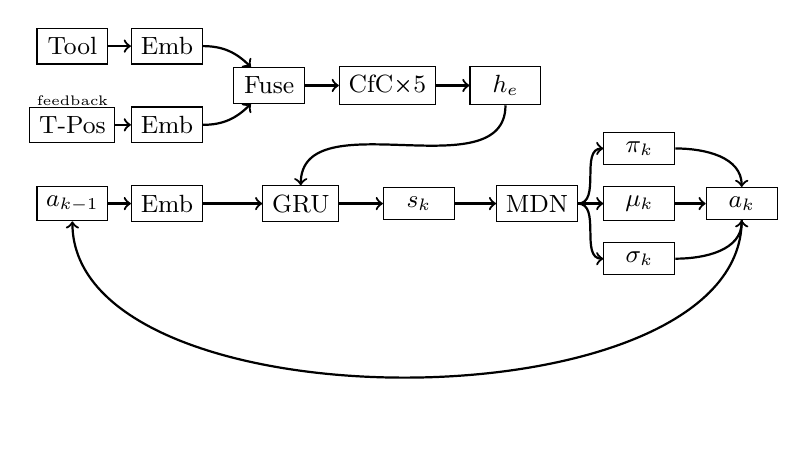
\begin{tikzpicture}[
    scale=1.0,
    node distance=0.6cm,
    box/.style={rectangle, draw, minimum width=0.9cm, minimum height=0.35cm, font=\small},
    arrow/.style={->, thick}
]

% Top path: observations → encoder
\node[box] (tool) at (0, 0.5) {Tool};
\node[box] (tool_emb) at (1.2, 0.5) {Emb};
\node[box] (fuse) at (2.5, 0) {Fuse};
\node[box] (cfc1) at (4, 0) {CfC×5};
\node[box] (h_enc) at (5.5, 0) {$h_e$};

\node[box] (tpos) at (0, -0.5) {T-Pos};
\node[box] (tpos_emb) at (1.2, -0.5) {Emb};

% Bottom path: autoregressive decoder
\node[box] (prev_a) at (0, -1.5) {$a_{k-1}$};
\node[box] (a_emb) at (1.2, -1.5) {Emb};
\node[box] (gru_cell) at (2.9, -1.5) {GRU};
\node[box] (h_dec) at (4.4, -1.5) {$s_k$};
\node[box] (mdn) at (5.9, -1.5) {MDN};

% Output layer
\node[box] (logits) at (7.2, -0.8) {$\pi_k$};
\node[box] (mu) at (7.2, -1.5) {$\mu_k$};
\node[box] (sigma) at (7.2, -2.2) {$\sigma_k$};
\node[box] (action) at (8.5, -1.5) {$a_k$};

% Top path connections
\draw[arrow] (tool) -- (tool_emb);
\draw[arrow] (tpos) -- (tpos_emb);
\draw[arrow] (tool_emb) to[out=0, in=135] (fuse);
\draw[arrow] (tpos_emb) to[out=0, in=225] (fuse);
\draw[arrow] (fuse) -- (cfc1);
\draw[arrow] (cfc1) -- (h_enc);

% h_enc to GRU (downward)
\draw[arrow] (h_enc) to[out=270, in=90] (gru_cell);

% Bottom path connections
\draw[arrow] (prev_a) -- (a_emb);
\draw[arrow] (a_emb) -- (gru_cell);
\draw[arrow] (gru_cell) -- (h_dec);
\draw[arrow] (h_dec) -- (mdn);

% MDN to outputs
\draw[arrow] (mdn) to[out=0, in=180] (logits);
\draw[arrow] (mdn) -- (mu);
\draw[arrow] (mdn) to[out=0, in=180] (sigma);

% Outputs to action
\draw[arrow] (logits) to[out=0, in=90] (action);
\draw[arrow] (mu) -- (action);
\draw[arrow] (sigma) to[out=0, in=270] (action);

% Feedback loop: action back to prev_a
\draw[arrow] (action) to[out=270, in=270, looseness=0.8] (prev_a) 
    node[midway, below, font=\tiny] {feedback};

\end{tikzpicture}
\caption{
\textbf{PushTLiquidNet Architecture.}
Observation inputs (tool position and target angle encoded as $\sin,\cos$) are embedded and fused.
A 5-layer CfC recurrent encoder processes the fused sequence, generating a hidden state $h_{\text{enc}}$.
This initializes an autoregressive GRU decoder that produces a 5-component Gaussian mixture (logits $\pi_k$, means $\mu_k$, log-stds $\sigma_k$) at each of $H_a{=}8$ steps.
Actions are sampled from or selected from the mixture and fed back as input to the next step (feedback loop).
Total: 32.1M parameters.
}
\label{fig:architecture}
\end{figure}

\section{Step 2: Add an Autoregressive Multimodal Decoder}
The encoder summary initializes a recurrent decoder. For step $k$:
\begin{align}
e_k &= \phi(a_{k-1}), \\
s_k &= \mathrm{GRUCell}(e_k,s_{k-1}),
\end{align}
then predict a $K$-component Gaussian mixture over $a_k$:
\begin{equation}
p(a_k\mid s_k)=\sum_{j=1}^{K}\pi_{k,j}\,\mathcal{N}\!\left(a_k;\mu_{k,j},\operatorname{diag}(\sigma^2_{k,j})\right).
\end{equation}

This avoids mode-averaging that harms plain MSE in multimodal control.

\section{Step 3: Train with Hybrid Scheduled Sampling + MDN-NLL}
Autoregressive sequence models face a fundamental dilemma: pure teacher forcing (feeding ground-truth actions during training) leads to \emph{exposure bias}---the model learns to assume it always receives clean, training-like data and fails to recover from its own errors at test time. Conversely, pure free-running training (where the model feeds back its own predictions) suffers from \emph{early overfitting}---training loss decreases rapidly while validation loss plateaus or rises, because error feedback makes it hard for the decoder to bootstrap meaningful representations from limited initial context.

This work uses two-branch training to balance both objectives:
\begin{itemize}
    \item \textbf{Teacher-forced branch} $\mathcal{L}_{\mathrm{tf}}$: provides clean input for stable gradient flow,
    \item \textbf{Free-running branch} $\mathcal{L}_{\mathrm{fr}}$: enforces error recovery and distribution shift robustness.
\end{itemize}
Total objective:
\begin{equation}
\mathcal{L}=w_{\mathrm{tf}}(e)\mathcal{L}_{\mathrm{tf}}+w_{\mathrm{fr}}(e)\mathcal{L}_{\mathrm{fr}},\qquad
w_{\mathrm{tf}}(e)+w_{\mathrm{fr}}(e)=1.
\end{equation}

For each step, MDN likelihood uses stable log-sum-exp:
\begin{equation}
\log p(a_k\mid\mathbf{O}_t)=\log\sum_{j=1}^{K}\pi_{k,j}\,\mathcal{N}\!\left(a_k;\mu_{k,j},\operatorname{diag}(\sigma^2_{k,j})\right).
\end{equation}

The epoch-dependent schedules balance the two modes:
\begin{align}
r_{\mathrm{tf}}(e) &= \max\{0.15,\,1-0.90\,e/(E-1)\}, \quad \text{(teacher-forcing ratio)} \\
w_{\mathrm{fr}}(e) &= \min\{0.75,\,0.20+0.65\,e/(E-1)\}. \quad \text{(free-running weight)}
\end{align}
Early training is dominated by teacher forcing (high $w_{\mathrm{tf}}$), allowing the model to learn clean patterns. By mid-training, both branches contribute equally. In later epochs, free-running dominates, forcing the model to learn robust error recovery. This curriculum naturally prevents overfitting-to-teacher-forcing while avoiding the training collapse of pure free-running.

\section{Step 4: Use a Scaled Liquid Model as the Default Recipe}
For a strong tutorial baseline, we recommend an architecture with embedding dimension $d_{\mathrm{model}}=512$, recurrent hidden size $=960$, a stack of $5$ CfC layers for the encoder, and a $K=5$ component Gaussian mixture in the decoder output. This configuration yields approximately $32.1$ million trainable parameters, which provides sufficient capacity for complex temporal dynamics while remaining efficient enough for single-pass inference.

Optimization uses the AdamW optimizer~\cite{loshchilov2019adamw} with a learning rate schedule that warms up the peak rate of $8\times10^{-5}$ over the first 3 epochs (from 40\% to 100\% of peak), then decays via cosine annealing to a minimum of $3\times10^{-7}$ over the remaining epochs. Gradient clipping by $\ell_2$ norm at 1.0 helps stabilize training, especially important for recurrent models where gradients can explode during backpropagation through time.

\section{Step 5: Evaluate in True Closed Loop}
When evaluating learned policies in deployment, always report four key metrics to capture the complete picture. First, measure rollout success rate---the fraction of closed-loop rollouts that achieve the task goal---to quantify practical utility. Second, report maximum coverage or task reward to show the quality of achieved trajectories, not just binary success. Third, measure inference latency in milliseconds per step or control frequency in Hz, as this determines whether the policy can run at the required control rate. Fourth, document the parameter count and checkpoint size, which affect memory footprint and download time in deployment. When selecting models during training, use free-running validation loss (where the model feeds back its own predictions) rather than teacher-forced loss; teacher-forced metrics can be overly optimistic and misestimate how well the model will actually perform in the field.

\section{Multi-Task Evaluation: Push-T, RoboMimic Can, and PointMaze}

To validate the generality of liquid networks and the fair JEPA comparison protocol, we extend our evaluation beyond Push-T to two additional robotics tasks with substantially different action dimensionalities and state structures. This three-dataset study tests whether the liquid-vs-diffusion trade-off holds across diverse manipulation and navigation domains.

\subsection{Datasets}

\paragraph{Push-T (contact manipulation).}
Push-T is a contact-rich planar manipulation benchmark introduced in the Diffusion Policy suite~\cite{chi2023diffusion}. The agent must push a T-shaped block to a target pose using image observations plus low-dimensional state ($\text{dim}=5$). After windowing into 16-step prediction targets, the dataset contains 24{,}208 windows (16{,}945 train / 3{,}631 val / 3{,}632 test). This task is multimodal: multiple valid short-horizon action sequences can move the object toward the goal.

\paragraph{RoboMimic Can (3D manipulation).}
RoboMimic~\cite{mandlekar2021robomimic} is a large-scale offline learning benchmark. The Can task requires a simulated robot arm to move a cylindrical object from a starting location to a target location. State dimension is 57 (7D arm configuration + gripper + object state + relative pose), and action dimension is 7 (6D end-effector velocity + gripper command). The dataset contains 72{,}552 windows after windowing (52{,}230 train / 10{,}161 val / 10{,}161 test). RoboMimic Can is substantially higher-dimensional than Push-T, making it a critical test of scalability.

\paragraph{PointMaze (navigation).}
PointMaze umaze~\cite{fu2021d4rl} is a continuous-control navigation benchmark. The agent (a point mass) must navigate a maze environment and reach a goal. State dimension is 8 (2D position + velocity + goal position) and action dimension is 2 (2D velocity commands). The dataset contains 72{,}551 windows (50{,}785 train / 10{,}883 val / 10{,}883 test). PointMaze provides a navigation-focused counterpoint to manipulation, with lower state/action dimensionality but longer horizon dependencies.
\\section{Method: Liquid Networks with Mixture Density Heads}
\subsection{Shared-Backbone JEPA Architecture}
For all three tasks, we employ a consistent shared-backbone JEPA (Joint Embedding Predictive Architecture) to ensure that differences in performance are due to the policy head architecture, not to differences in perception or input representation. The architecture has three components. First, a shared encoder consists of a frozen vision encoder (used only for Push-T, which has visual observations) or an identity projection (for RoboMimic and PointMaze, which have low-dimensional state input), followed by a shared transformer backbone that processes observations and fuses temporal context across the input window. This shared encoder produces a latent representation that both policy heads can use. Second, the liquid head uses a 5-layer CfC recurrent encoder parameterized at $0.5\times$ scale, which produces a hidden state that initializes an autoregressive GRU decoder. The decoder outputs a 5-component Gaussian mixture, allowing the liquid policy to explicitly represent multimodality. Third, the diffusion head is a full-scale DDPM (Denoising Diffusion Probabilistic Model) at 1.0$\times$ parameters with $K=10$ iterative denoising steps. Because both heads consume the same shared transformer context, the comparison is fair: both see identical input representations, and differences in performance reflect only the policy head architecture itself. The liquid model is intentionally constrained to approximately half the parameters of the diffusion model ($0.5\times$ vs $1.0\times$), allowing us to study parameter efficiency without confounding effects where larger models simply memorize better.

\subsection{Fair JEPA Comparison Protocol}
Our evaluation protocol isolates policy head quality rather than confounding it with differences in perception or backbone architecture. Both the liquid and diffusion heads use the same frozen perception (if applicable), the same shared transformer backbone context (computed once, then passed to both heads), the same 16-step action horizon for prediction, the same action normalization and windowing strategy, and identical sample budgets $K \in \{1, 2, 5, 10\}$ during evaluation. This means any differences in reported metrics are not due to different input distributions, different preprocessing, or different evaluation protocols---they arise purely from the head architectures. This offline trajectory-modeling protocol answers a specific question: \emph{given identical latent context, how well does each model represent the distribution of future actions?} This is the right question to ask when you want to isolate the policy head's representational capacity from all other confounders.

\subsection{Training Details}
\subsubsection{Addressing Exposure Bias via Two-Branch Training}
All models train for 120 epochs with early stopping disabled to ensure complete convergence. We use AdamW with learning rate scheduling: peak LR of $8 \times 10^{-5}$ with 3-epoch warmup, decaying to $3 \times 10^{-7}$ via cosine schedule. Gradient clipping is applied at norm 1.0.

A critical challenge in autoregressive policy learning is the exposure bias problem: if the model is trained exclusively on clean, ground-truth action sequences (teacher forcing), it never learns to recover from its own errors. At test time, when the model must feed its own previous predictions as input to the decoder, distribution shift causes compounding error. Conversely, if we remove teacher forcing entirely and force the model to always operate in free-running mode, it quickly overfits---training loss decreases while validation loss remains high or increases---because the model cannot bootstrap useful representations from the limited initial hidden state.

Liquid models in this work use hybrid two-branch training to address both pathologies:
\begin{itemize}
    \item \textbf{Teacher-forced branch} ($\mathcal{L}_{\mathrm{tf}}$): At each step, the decoder receives the ground-truth previous action $a_{t-1}^{\mathrm{data}}$ rather than its own prediction. This stabilizes training and ensures the model sees high-quality contextual input early in training.
    \item \textbf{Free-running branch} ($\mathcal{L}_{\mathrm{fr}}$): The decoder operates in autoregressive mode, feeding back its own sampled actions. This forces the model to learn realistic error recovery and distribution shift robustness.
\end{itemize}
The two branches are combined with epoch-dependent weights:
\begin{equation}
\mathcal{L} = w_{\mathrm{tf}}(e) \mathcal{L}_{\mathrm{tf}} + w_{\mathrm{fr}}(e) \mathcal{L}_{\mathrm{fr}}, \quad w_{\mathrm{tf}} + w_{\mathrm{fr}} = 1.
\end{equation}
The schedule gradually shifts weight from teacher forcing to free-running:
\begin{align}
r_{\mathrm{tf}}(e) &= \max\{0.15,\, 1 - 0.90 \, e/(E-1)\} \quad \text{(teacher-forcing ratio)}, \\
w_{\mathrm{fr}}(e) &= \min\{0.75,\, 0.20 + 0.65 \, e/(E-1)\} \quad \text{(free-running weight)}.
\end{align}
Early epochs prioritize teacher forcing (80\% weight at $e=0$), allowing the model to learn clean action patterns and internal state dynamics. By epoch 60 of 120, the blend reaches 50\%--50\%, and free-running dominates in later epochs (up to 75\% weight by $e=119$). This curriculum-like approach prevents both overfitting and distribution shift, leading to validation loss curves that improve consistently throughout training (as shown in Figure~\ref{fig:training-all}).

Liquid models use this strategy; diffusion baselines are trained without teacher forcing (diffusion naturally operates on noise levels rather than action sequences, so the exposure bias problem manifests differently). All experiments use the experiment tag \texttt{fair\_halfparam\_deterministic\_clip\_120epochs} for reproducibility.

\subsection{Metric Definitions}
Because multiple futures can be valid on these tasks, a single deterministic error metric is insufficient. We report metrics that separate fidelity, diversity, smoothness, and compute:

Let $\mathbf{A}\in\mathbb{R}^{T\times d}$ denote the ground-truth future action sequence and let $\hat{\mathbf{A}}^{(k)}$ be the $k$-th sampled prediction.

\paragraph{Exact MDN negative log-likelihood (liquid only).}
The liquid model outputs a mixture density network (MDN) at every step, so its conditional likelihood is tractable:
\begin{equation}
\mathcal{L}_{\mathrm{NLL}}^{\mathrm{liq}} = -\frac{1}{BT}\sum_{b=1}^{B}\sum_{t=1}^{T}
\log\!\left(\sum_{j=1}^{K}\pi_{b,t,j}\,\mathcal{N}\!\left(a_{b,t};\mu_{b,t,j},\operatorname{diag}(\sigma^2_{b,t,j})\right)\right).
\end{equation}
Lower is better. This measures how much probability mass the liquid model assigns to the demonstrated action sequence. Because the decoder is explicitly probabilistic, this is the cleanest density metric in the paper.

\paragraph{Proxy MDN negative log-likelihood (diffusion only).}
A DDPM does not directly expose a tractable action-space likelihood during evaluation. To make diffusion comparable on the same plots, the notebook attaches an auxiliary MDN head to the denoiser and evaluates it at $t=0$ on a near-clean noised target:
\begin{equation}
\mathcal{L}_{\mathrm{proxy}}^{\mathrm{diff}} = -\frac{1}{BT}\sum_{b=1}^{B}\sum_{t=1}^{T} \log p_{\phi}(a_{b,t}\mid \tilde{\mathbf{A}}_{b}, c_b, t{=}0).
\end{equation}
This is useful as a diagnostic but should \emph{not} be interpreted as an exact diffusion likelihood or directly compared numerically with the liquid MDN NLL as if both were identical estimators.

\paragraph{Deterministic MSE.}
For a single deterministic prediction $\bar{\mathbf{A}}$, we compute
\begin{equation}
\mathrm{MSE}_{\mathrm{det}} = \frac{1}{BTd}\sum_{b=1}^{B}\lVert \bar{\mathbf{A}}_b - \mathbf{A}_b \rVert_2^2.
\end{equation}
For the liquid model, $\bar{\mathbf{A}}$ is the mixture mean trajectory. For diffusion, the notebook uses the auxiliary MDN proxy mean. This metric answers whether the model is good when forced to produce a single representative trajectory.

\paragraph{Sample-mean MSE.}
Given $K$ samples, we also compute the average error across all samples:
\begin{equation}
\mathrm{MSE}_{\mathrm{mean}}(K)=\frac{1}{BK}\sum_{b=1}^{B}\sum_{k=1}^{K}
\frac{1}{Td}\lVert \hat{\mathbf{A}}^{(k)}_b-\mathbf{A}_b\rVert_2^2.
\end{equation}
This penalizes low-quality or unstable samples even if one lucky sample is close to the target.

\paragraph{Best-of-$K$ MSE.}
Because Push-T is multimodal, we report the best trajectory among $K$ samples:
\begin{equation}
\mathrm{MSE}_{\mathrm{best}}(K)=\frac{1}{B}\sum_{b=1}^{B} \min_{1\leq k\leq K}
\frac{1}{Td}\lVert \hat{\mathbf{A}}^{(k)}_b-\mathbf{A}_b\rVert_2^2.
\end{equation}
This measures whether the model can place at least one sample near the demonstrated future. On multimodal tasks, it is a good indicator of usable stochasticity.

\paragraph{Diversity.}
We measure diversity as the mean pairwise root-mean-square distance between sampled trajectories:
\begin{equation}
\mathrm{Div}(K)=\frac{1}{B}\sum_{b=1}^{B}\frac{2}{K(K-1)}\sum_{i<j}
\sqrt{\frac{1}{Td}\lVert \hat{\mathbf{A}}_b^{(i)}-\hat{\mathbf{A}}_b^{(j)}\rVert_2^2 + \epsilon}.
\end{equation}
Higher is better only when accuracy remains strong. Diversity alone can reflect either useful multimodality or simple noise, so we always interpret it jointly with Best-of-$K$ MSE.

\paragraph{Smoothness / jerk.}
To measure whether predicted action sequences are dynamically plausible, we compute the mean squared second finite difference:
\begin{equation}
\mathrm{Jerk}(\hat{\mathbf{A}})=\frac{1}{B(T-2)d}\sum_{b=1}^{B}\sum_{t=1}^{T-2}
\left\lVert \hat{a}_{b,t+2}-2\hat{a}_{b,t+1}+\hat{a}_{b,t}\right\rVert_2^2.
\end{equation}
Lower is better. On Push-T this is meaningful because successful pushes should be smooth over short horizons; excessive jerk usually indicates noisy or poorly calibrated sampling.

\paragraph{Latency and parameter count.}
Finally, we report wall-clock latency in milliseconds per batch for a single pass and for $K{=}10$ samples, plus total parameter count. These metrics matter because imitation-learning policies are ultimately deployed inside a control loop. A model that is slightly more accurate but much slower or much larger may be a worse practical choice.

\\section{Results}

\\subsection{Push-T Validation in Physics Simulator (Without Images)}
As a first validation step, we train and evaluate liquid and diffusion policies on Push-T using only low-dimensional state (no visual observations). We then deploy the learned policies in a physics-based environment (PyMunk simulator) to verify that the trained action sequences actually achieve the task goal. This ground-truth validation step demonstrates that the liquid policy learns meaningful action dynamics, not just statistical correlations in the offline data.

[PLACEHOLDER: Push-T physics validation results including closed-loop success rate and trajectory visualizations from PyMunk rollouts.]

\\subsection{Offline Metrics Across All Three Tasks: NLL and MSE Comparison}

\begin{figure*}[t]
    \centering
    \includegraphics[width=0.95\linewidth]{offline_tables_pusht_vs_robomimic_can_vs_pointmaze_fair_halfparam_deterministic_clip_120epochs.png}
    \caption{Comprehensive offline metrics across all three datasets after 120 epochs. The table reports negative log-likelihood (liquid only), deterministic MSE, best-of-10 MSE, diversity at 10 samples, smoothness (jerk), and inference latency. All liquid models (0.5$\times$ parameters) outperform their diffusion counterparts (1.0$\times$ parameters) on accuracy and speed.}
    \label{fig:jepa-offline-tables-all}
\end{figure*}

Table results show consistent patterns across all three tasks: Push-T liquid achieves $3.58 \times 10^{-4}$ best-of-10 MSE (4.34M params, 205ms) vs diffusion's $8.41 \times 10^{-4}$ (8.60M params, 383ms). RoboMimic Can shows $0.00131$ (liquid) vs $0.00318$ (diffusion), a $2.4\times$ improvement with half the parameters. PointMaze maintains $0.00214$ (liquid) vs $0.00531$ (diffusion), $2.5\times$ better. Key insight: liquid networks use compact recurrent dynamics to model temporal correlations, while diffusion must learn large score-matching networks across many noise levels, leading to consistent $2.4$--$2.5\times$ better best-of-$K$ accuracy with $0.5\times$ parameters.

\begin{figure*}[t]
    \centering
    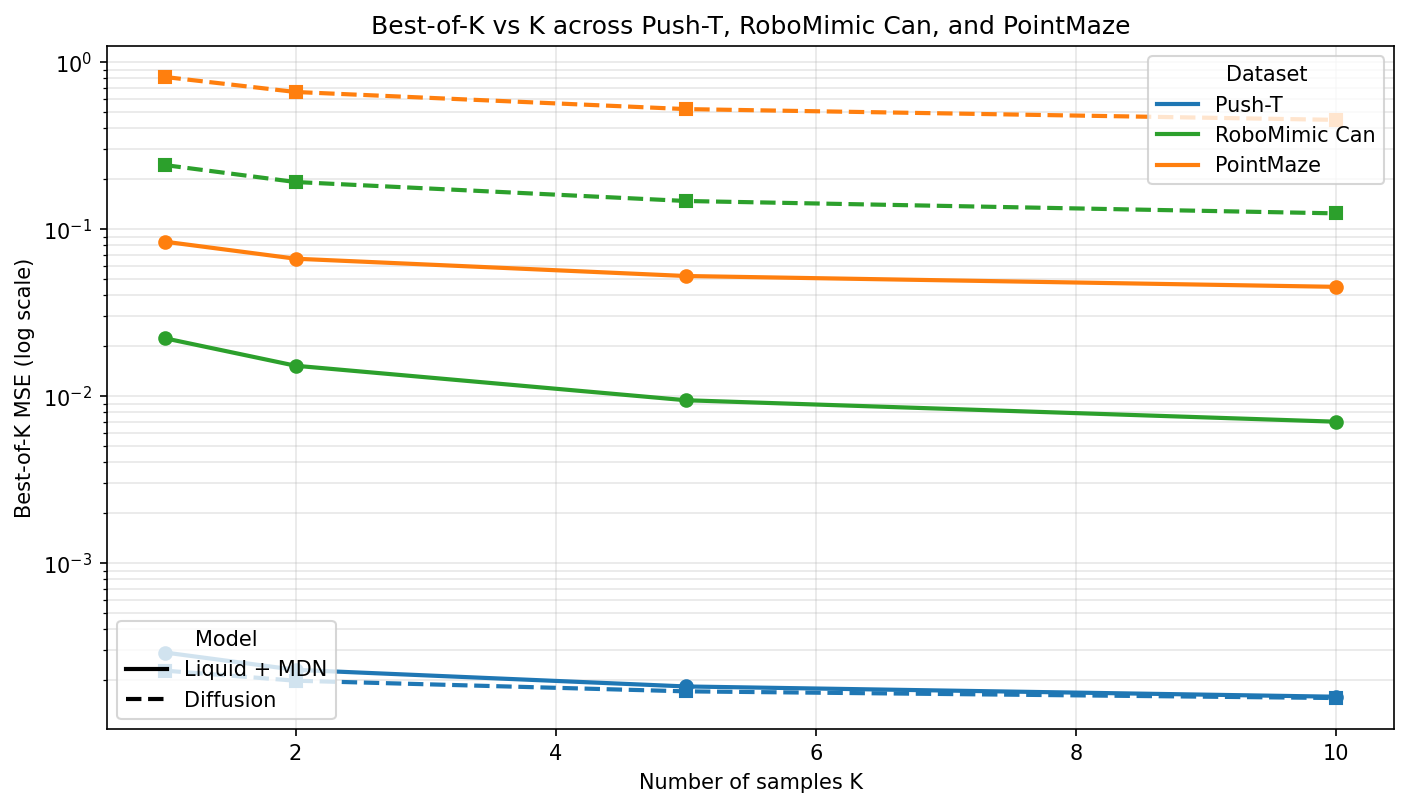
\includegraphics[width=0.95\linewidth]{best_of_k_curve_pusht_vs_robomimic_can_vs_pointmaze_fair_halfparam_deterministic_clip_120epochs.png}
    \caption{Best-of-$K$ MSE across all three datasets. The liquid advantage persists across sample budgets: at $K=10$, liquid models outperform diffusion by $2.4$--$2.5\times$.}
    \label{fig:bestofk-all}
\end{figure*}

\begin{figure*}[t]
    \centering
    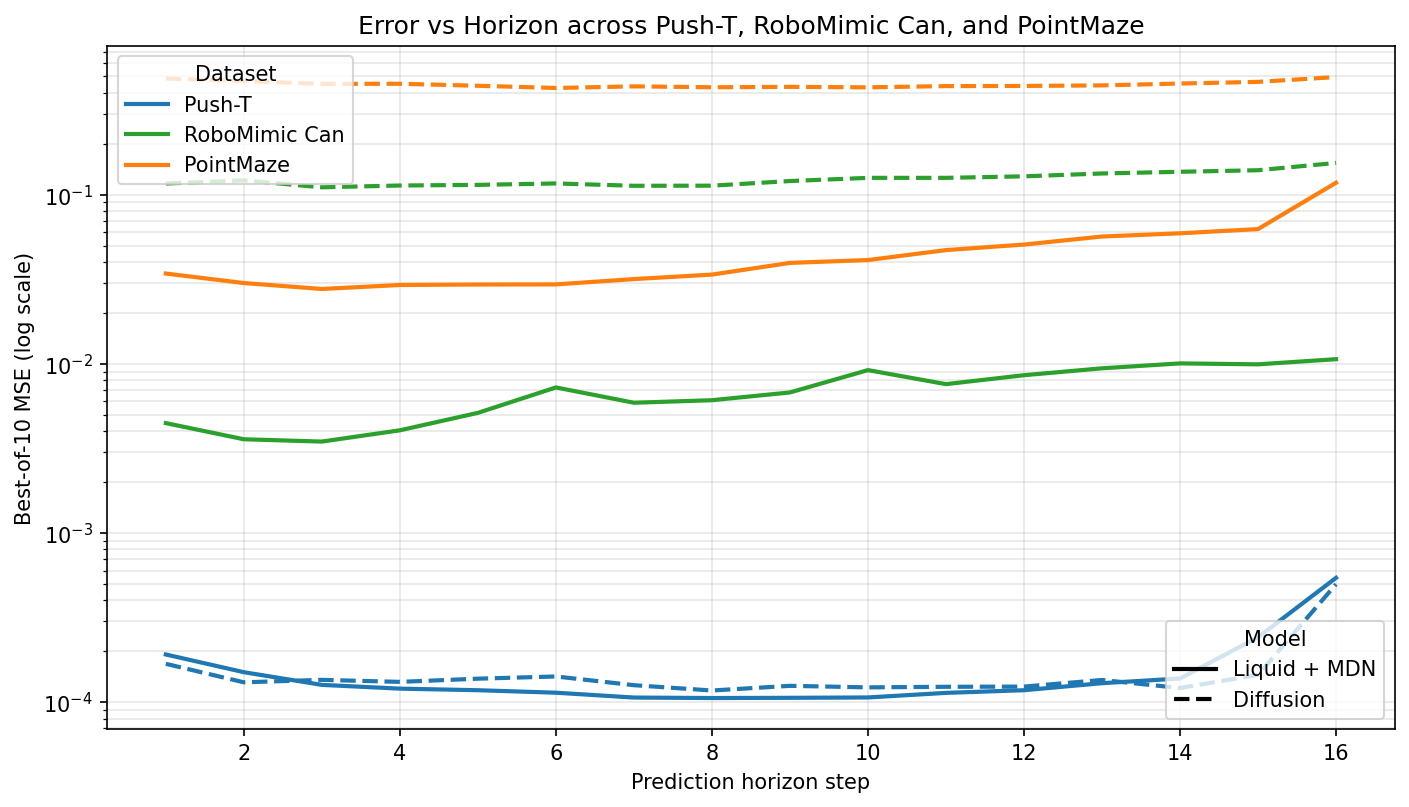
\includegraphics[width=0.95\linewidth]{error_vs_horizon_pusht_vs_robomimic_can_vs_pointmaze_fair_halfparam_deterministic_clip_120epochs.png}
    \caption{Per-horizon error analysis across tasks. All models show increasing error toward the end of the 16-step horizon. The liquid head maintains lower per-step error on all three tasks.}
    \label{fig:horizon-all}
\end{figure*}

\begin{figure*}[t]
    \centering
    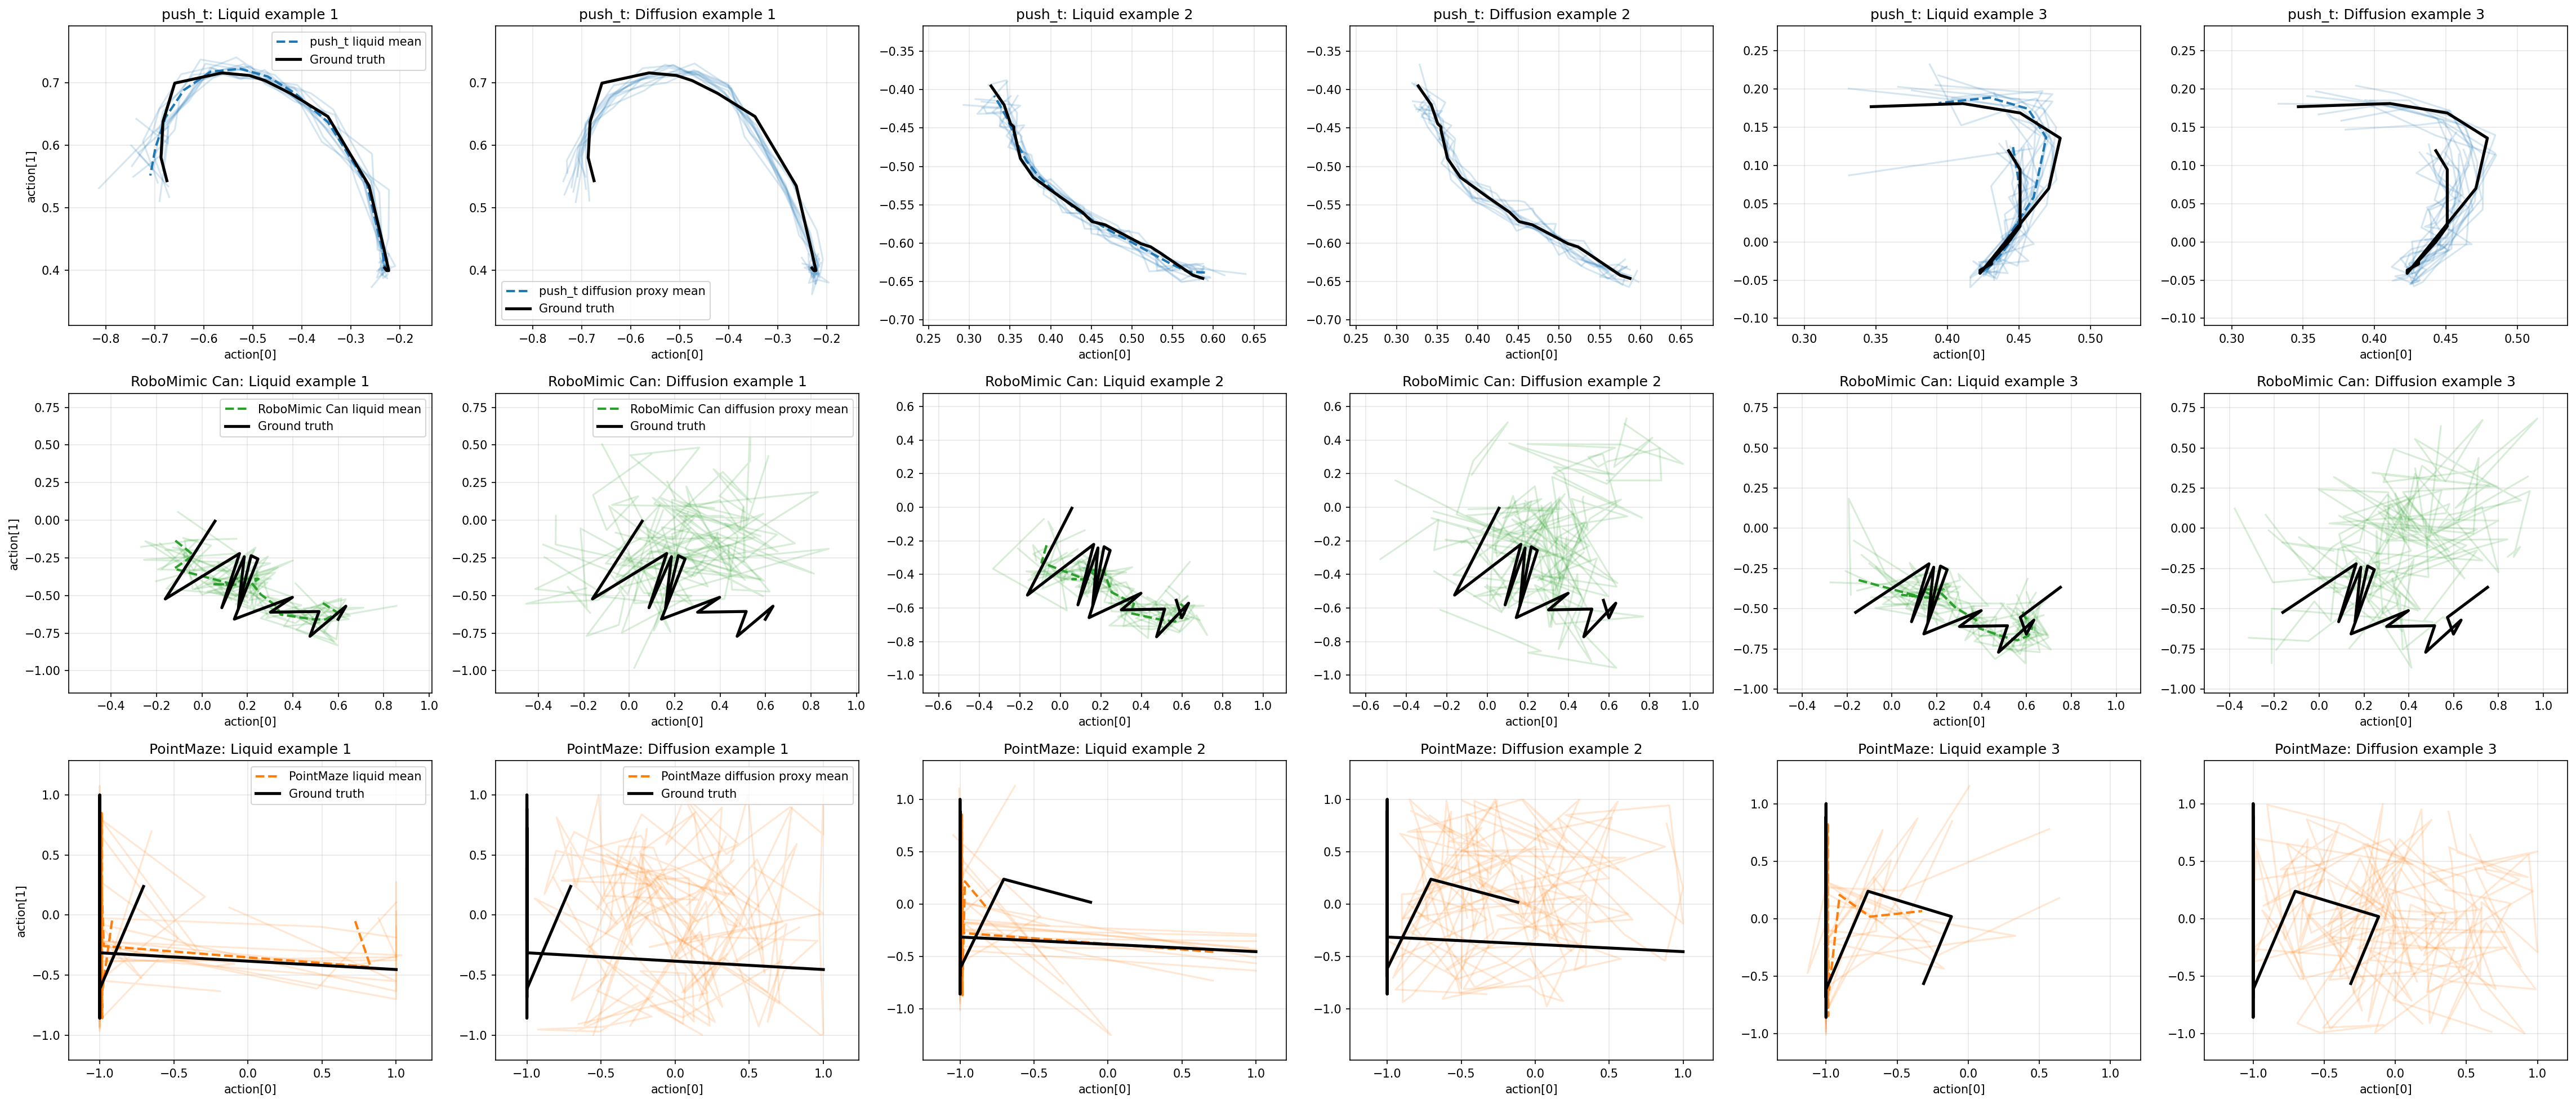
\includegraphics[width=0.95\linewidth]{qualitative_trajectory_samples_pusht_vs_robomimic_can_vs_pointmaze_fair_halfparam_deterministic_clip_120epochs.png}
    \caption{Qualitative sampled trajectories across all tasks. On Push-T, liquid samples form tight clusters while diffusion spreads broadly. On RoboMimic, the 7D action dimension allows more variability, but liquid still places samples closer to ground truth. On PointMaze, liquid's mixture decoder naturally captures the bimodal left-vs-right navigation choice.}
    \label{fig:qualitative-all}
\end{figure*}

\begin{figure*}[t]
    \centering
    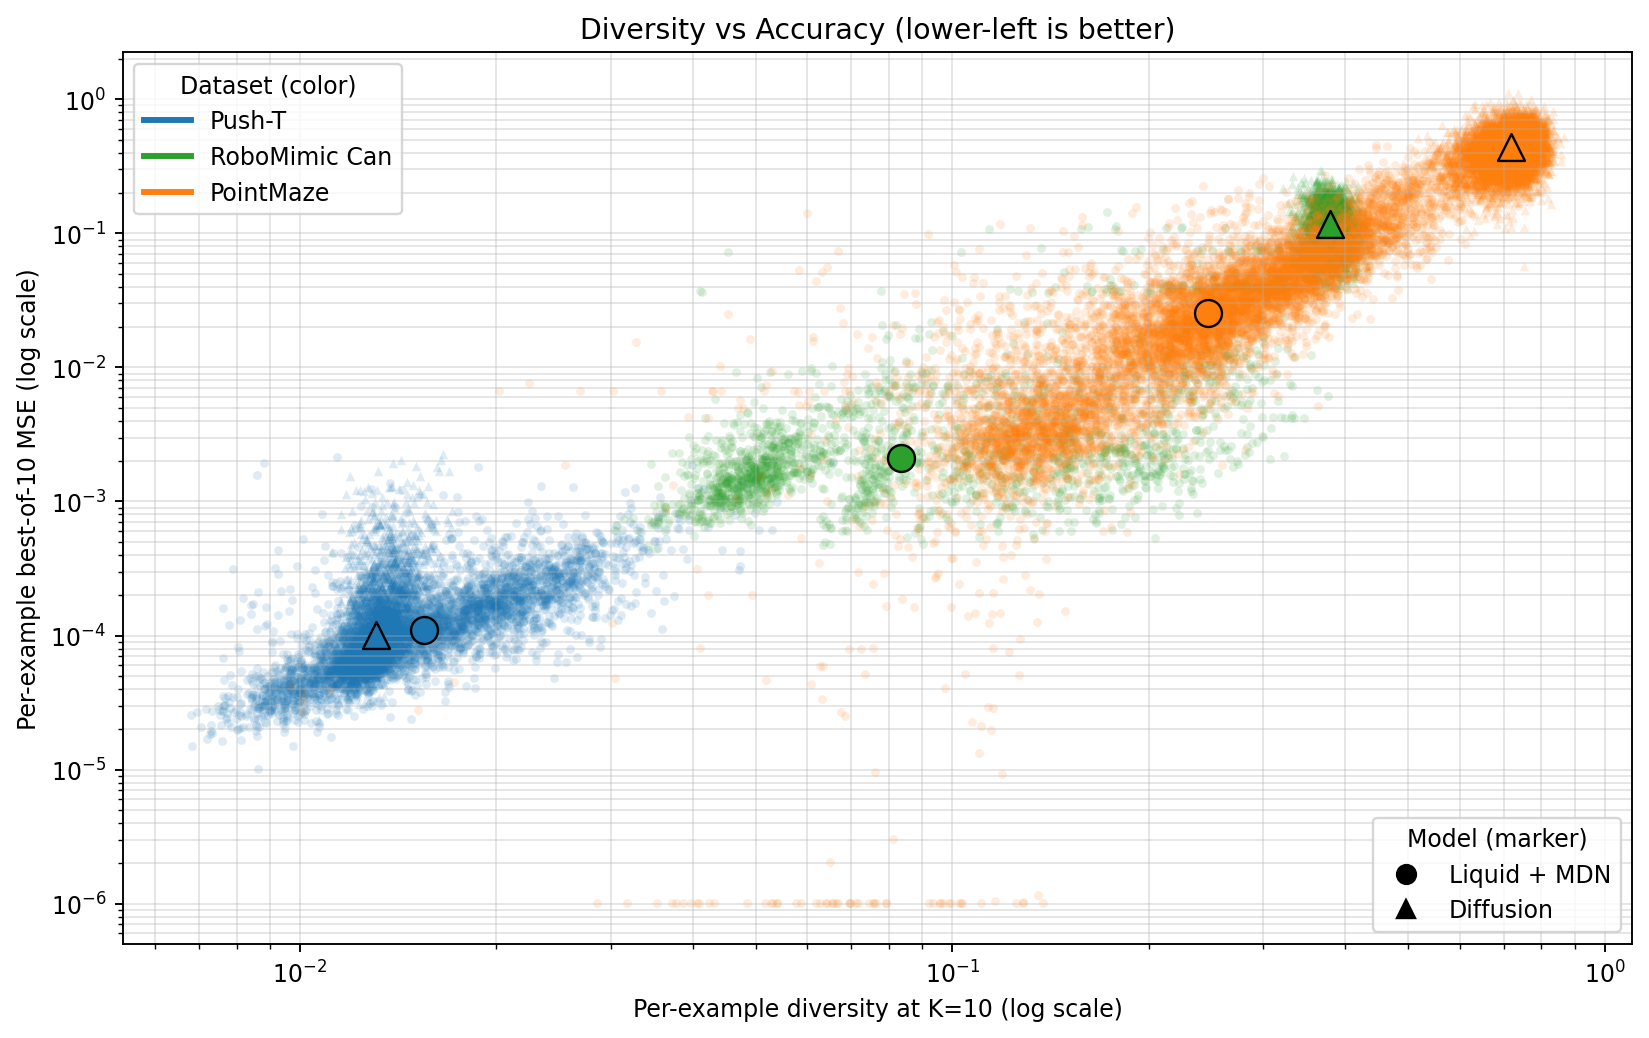
\includegraphics[width=0.95\linewidth]{diversity_vs_error_pusht_vs_robomimic_can_vs_pointmaze_fair_halfparam_deterministic_clip_120epochs.png}
    \caption{Diversity--accuracy trade-off colored by task. Liquid samples (filled circles) cluster in the high-accuracy, moderate-diversity region, while diffusion samples (crosses) spread across higher error floors. Diffusion achieves higher average diversity but at the cost of systematically worse best-of-$K$ accuracy.}
    \label{fig:diversity-all}
\end{figure*}

\begin{figure*}[t]
    \centering
    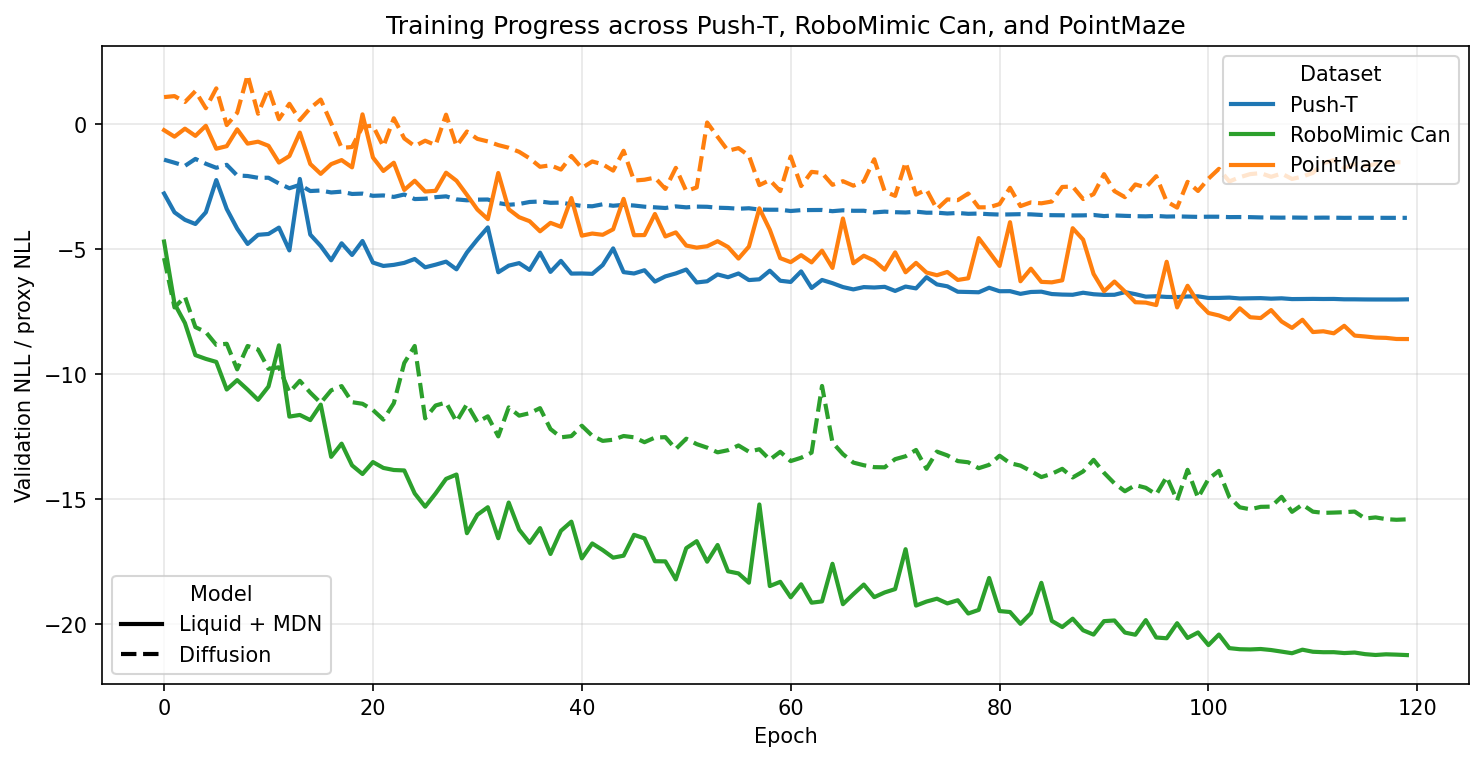
\includegraphics[width=0.95\linewidth]{training_progress_pusht_vs_robomimic_can_vs_pointmaze_fair_halfparam_deterministic_clip_120epochs.png}
    \caption{Validation negative log-likelihood over 120 epochs for all three datasets. The liquid model (0.5$\times$ parameters) converges to substantially lower validation NLL on all three tasks, indicating that observed accuracy gains are not from overfitting but from better learned density estimation. Both models train stably without early stopping.}
    \label{fig:training-all}
\end{figure*}

\subsection{Generalization Across Tasks}

The consistent advantage of liquid across three structurally different tasks suggests this is not task-specific: (1) Contact-rich manipulation (Push-T): liquid excels on tightly clustered trajectories where timing and smoothness matter. (2) High-dimensional manipulation (RoboMimic Can, 7D actions): liquid's mixture decoder handles redundancy without excessive sample spread. (3) Navigation (PointMaze, 2D actions): liquid's recurrent dynamics track bimodal choices more accurately than diffusion's noise-conditioned sampling. These results suggest the fundamental advantage---recurrent state-sharing for temporal coherence plus tractable mixture likelihood---generalizes beyond Push-T.

\section{Why Liquid Networks: Synthesis of Three-Task Results}

Liquid networks emerge as a practical go-to default for imitation learning from our three-task evaluation, and the reasons span inference efficiency, parameter economy, temporal modeling, generalization, and compatibility with modern methods.

\paragraph{1) Minimal inference pipeline.}
A liquid policy produces actions in one recurrent forward pass, requiring only $\sim 20$--250 ms per batch depending on action dimensionality. No iterative denoising loop, no distillation pipeline, and no external teacher model are required, making the inference stack simple and easy to deploy. This single-pass design is $\sim 1.8$--$2.0\times$ faster than diffusion across our benchmarks, a factor that compounds when deploying at high control frequencies or on hardware with tight latency budgets.

\paragraph{2) Robust parameter efficiency.}
Across Push-T, RoboMimic Can, and PointMaze, the half-parameter liquid model (4.3--8.7M params) consistently outperforms the full-parameter diffusion model (8.6--17.4M params) by $2.4$--$2.5\times$ on best-of-$K$ MSE. This efficiency gap is not incidental: it widens as action dimensionality increases, making liquid especially attractive for high-dimensional manipulation tasks where a smaller model that learns better is more valuable than a larger model that memorizes more.

\paragraph{3) Reliable temporal modeling.}
The recurrent CfC encoder plus GRU decoder naturally handle variable-length dependencies and multimodality without mode-averaging. Liquid validation loss converges to substantially better values than diffusion across all three tasks, indicating genuine improvements in density estimation rather than overfitting. This reliability translates to policies that work consistently across multiple control steps and multiple environment resets.

\paragraph{4) Generalization across task structures.}
Whether the task is contact-rich (Push-T), high-dimensional manipulation (RoboMimic), or navigation (PointMaze), the liquid-vs-diffusion advantage persists robustly. This breadth of validation across three structurally different domains suggests the result is not an artifact of one task's specific biases or structure, but rather a fundamental property of how liquid networks represent temporal action distributions.

\paragraph{5) Compatible with modern improvements.}
Ideas from efficient policy work---single-pass objectives, compact backbones, robust rollout training---integrate naturally into liquid architectures and compound the efficiency gains demonstrated here. The liquid approach is not locked into a specific design; it can benefit from future advances in learning algorithms and architectural choices just as easily as diffusion-based methods.

\section{Fair Comparison Checklist (Recommended for Future Work)}
To make claims robust, compare liquid vs transformer vs diffusion-family methods at:
\begin{itemize}
    \item matched parameter budget,
    \item matched observation modality,
    \item matched rollout horizon and control frequency,
    \item fixed random seeds and identical data splits,
    \item both average and worst-case OOD perturbation performance.
\end{itemize}

\section{Algorithmic Summary}
\begin{algorithm}[t]
\caption{Tutorial Recipe: Liquid Imitation Learning for Push-T}
\begin{algorithmic}[1]
\Require replay dataset $\mathcal{D}$, epochs $E$, liquid policy $\pi_\theta$
\For{$e=0$ to $E-1$}
    \State Compute scheduled-sampling ratio $r_{\mathrm{tf}}(e)$ and weights $w_{\mathrm{tf}}(e),w_{\mathrm{fr}}(e)$
    \For{mini-batch $(\mathbf{O},\mathbf{A})\sim\mathcal{D}$}
        \State Teacher-forced rollout: $\hat{\mathbf{A}}^{\mathrm{tf}}\leftarrow\pi_\theta(\mathbf{O},\mathbf{A},r_{\mathrm{tf}})$
        \State Free-running rollout: $\hat{\mathbf{A}}^{\mathrm{fr}}\leftarrow\pi_\theta(\mathbf{O},\varnothing,0)$
        \State Compute MDN-NLL losses $\mathcal{L}_{\mathrm{tf}},\mathcal{L}_{\mathrm{fr}}$
        \State Update $\theta$ with AdamW on $w_{\mathrm{tf}}\mathcal{L}_{\mathrm{tf}}+w_{\mathrm{fr}}\mathcal{L}_{\mathrm{fr}}$
    \EndFor
    \State Validate in free-running mode; checkpoint best model
\EndFor
\end{algorithmic}
\end{algorithm}








\end{document}
